%===============================================================================
% Zweck:    KTR-Seminar-Vorlage
% Erstellt: 16.10.2007
% Updated:  15.04.2013
% Autor:    U.K. / M.G.
%===============================================================================

%===============================================================================
% Zum Kompilieren pdflatex und bibtex ausführen.
%	Konfiguration: in texmaker unter Benutzer -> Benutzerbefehle einen neuen Befehl anlegen: pdflatex -synctex=1 -interaction=nonstopmode %.tex | bibtex % | makeindex %.nlo -s nomencl.ist -o %.nls | pdflatex -synctex=1 -interaction=nonstopmode %.tex | pdflatex -synctex=1 -interaction=nonstopmode %.tex
%	Entsprechende Informationen in den config/metainfo verändern
% Zur Auswahl der Sprache im folgenden Befehl
% ngerman für deutsch eintragen, english für Englisch.
%===============================================================================

% Options ngerman, english
\newcommand{\lang}{english}

\documentclass[pdftex, journal, onecolumn, a4paper, 12pt, \lang]{IEEEtran}

%===============================================================================
% zentrale Layout-Angaben und Befehle
%===============================================================================
% What You should change:
% Here goes your name
\author{Mahalakshmi Suravarapu}
% and the title of your seminar
\newcommand{\subtitle}{Fog Computing}
% the date of the submission
\date{October 06, 2020}

% What is already done
\newcommand{\semester}{\ifthenelse{\equal{\lang}{ngerman}}{Sommersemester 2020}{Summer Term 2020}}
\title{\ifthenelse{\equal{\lang}{ngerman}}{Fog Computing in Next Generation Networks}{%
Fog Computing in Next Generation Networks
}}\newcommand{\supervisor}{Prof. Dr. Udo Krieger}
%\institute[shortinstitute]{Institute}

%\titlegraphic{
\includegraphics[width=13mm,height=13mm]{image/logo}}
%\subject{subject}
%\keywords{keywords}

%===============================================================================
% Zweck: KTR-Seminar-Vorlage in Anlehung an G. Wirtz, Lehrstuhl Praktische Informatik
%===============================================================================
%===============================================================================
% zentrale Layout-Angaben und Befehle
%===============================================================================
%
% \usepackage{german}
\usepackage{ifthen}
% Language Selection for Babel
\ifthenelse{\equal{\lang}{ngerman}}{\usepackage[german, \lang]{babel}}{\usepackage[\lang]{babel}}

\usepackage[utf8]{inputenc}
\usepackage{fancyhdr}
\usepackage[T1]{fontenc}
\usepackage{ae}
\usepackage{color}
\usepackage{amsmath}
\usepackage{amsfonts}
%

\usepackage{caption}

%%   Fuer anspruchsvolle Tabellen   %%
\usepackage{longtable, colortbl}
\usepackage{multicol, multirow}

\usepackage[pdftitle={\@title},pdfauthor={\@author},pdftex,bookmarksopen,bookmarksnumbered,pdfborder=0]{hyperref}
\usepackage[pdftex]{graphicx}
\usepackage{float}
\usepackage{tikz}
\usepackage{pgfplots}
\usetikzlibrary{arrows,shapes,fit,positioning,snakes,backgrounds,shadows}

\pdfcompresslevel=9

% Code-Hervorhebung
% Quellcode
\usepackage{verbatim}            % Quellcode einbinden (\verbatiminput) standardpaket
\usepackage{moreverb} 
% PseudoCode
\usepackage{algorithm}
\usepackage{algpseudocode}
%\usepackage{algorithmicx}
\floatname{algorithm}{Algorithmus}
\algrenewcommand{\algorithmiccomment}[1]{\hskip1em\textcolor{gray!60}{$\rhd$ #1}}
\ifthenelse{\equal{\lang}{ngerman}}{%
\renewcommand{\listalgorithmname}{Algorithmen}
\def\algorithmautorefname{Algorithmus}
}{%
\renewcommand{\listalgorithmname}{List of Algorithms}
\def\algorithmautorefname{Algorithm}
}


%%   intoc zur Aufnhame des Abkuerzungs- und Symbolverzeichnisses ins Inhaltsverzeichnis  
\usepackage[intoc]{nomencl}
\setlength{\nomlabelwidth}{.20\hsize}
%\renewcommand{\nomlabel}[1]{#1 \dotfill}
\setlength{\nomitemsep}{-\parsep}
\makenomenclature
\ifthenelse{\equal{\lang}{ngerman}}{%
\renewcommand{\nomname}{Abk\"urzungsverzeichnis}
%\newcommand{\nomaltname}{Symbolverzeichnis}
}{%
\renewcommand{\nomname}{List of Abbreviations}
%\newcommand{\nomaltname}{List of Symbols}
}%
%\newcommand{\nomaltpreamble}{}
%\newcommand{\nomaltpostamble}{}
%\newcommand{\usetwonomenclatures}{\nomenclature[\switchnomitem]{}{}}
%\newcommand{\switchnomitem}{R}
%\renewcommand{\nomgroup}[1]{%
%\ifthenelse{\equal{#1}{\switchnomitem}}{\switchnomalt}{}}
%\newcommand{\switchnomalt}{%
%\end{thenomenclature}
%\newpage
%\renewcommand{\nomname}{\nomaltname}
%\renewcommand{\nompreamble}{\nomaltpreamble}
%\renewcommand{\nompostamble}{\nomaltpostamble}
%\begin{thenomenclature}
%}


%%   Hervorhebung der Abkuerzungsbuchstaben   %%
\usepackage[normalem]{ulem}
\newcommand{\m}[1]{\uline{#1}}

%\usepackage[dvips]{rotating}
%
% ausf\"{u}hrlichere Fehlermeldungen
\errorcontextlines=999
%
% Page-Layout: A4 aus Header
% Alternative
\setlength\headheight{14pt}
\setlength\topmargin{-15,4mm}
\setlength\oddsidemargin{-0,4mm}
\setlength\evensidemargin{-0,4mm}
\setlength\textwidth{160mm}
\setlength\textheight{252mm}
%
%% Absatzeinstellungen
\setlength\parindent{0mm}
\setlength\parskip{2ex}


\makeatletter
\renewcommand{\maketitle} {
  \begin{titlepage}
  \centering
    \begin{minipage}[t]{16cm}
      \hfill
      \begin{minipage}{12cm}
      \ifthenelse{\equal{\lang}{ngerman}}{%
        \centering
        Otto-Friedrich-Universit\"at Bamberg
        \\[12pt]%
        {\Large Professur f\"ur Informatik\\[.5em]%
        \large insbesondere Kommunikationsdienste,\\[.5em]%
        Telekommunikationsdienste und Rechnernetze}%
        }{%
        \centering
        Otto-Friedrich-University of Bamberg
        \\[12pt]
        {\Large Professorship for Computer Science,\\[.5em]%
        \large Communication Services, Telecommunication\\[.5em]%
        Systems and Computer Networks}%
        }
      \end{minipage}
      \hfill
      \begin{minipage}{3cm}
        
\includegraphics[height=28mm]{config/images/logo} %height=26mm
      \end{minipage}
    \end{minipage}\\[70pt]%[50pt]
   % 
    {\Large\bf \ifthenelse{\equal{\lang}{ngerman}}{Ausarbeitung des KTR-Seminars}{Seminar on}}
    \\[36pt]
   % oder: {\LARGE Ausarbeitung des KTR-Seminars}\\[12pt]
    {\LARGE \@title}\\[80pt]
    {\Large\bf \ifthenelse{\equal{\lang}{ngerman}}{Thema:}{Topic:}}\\[36pt]
    {\LARGE\bf \subtitle}\\
    \vfill
    \begin{minipage}{\textwidth}
      \center
      \ifthenelse{\equal{\lang}{ngerman}}{Vorgelegt von:}{Submitted by:}\\
      {\Large \@author \\[18pt]}
      \ifthenelse{\equal{\lang}{ngerman}}{Betreuer:}{Supervisor:} \supervisor \\[12pt]
      Bamberg, \@date\\
      \semester
    \end{minipage}
  \end{titlepage}
}
\makeatother
%
\usepackage[intoc]{nomencl}
\ifthenelse{\equal{\lang}{ngerman}}{%
\renewcommand{\nomname}{Abkürzungsverzeichnis}}%
{\renewcommand{\nomname}{List of Abbreviations}}
\renewcommand{\nomlabel}[1]{#1 \dotfill}
\makenomenclature

% Einbindung eines Bildes mit angegebener Breite
% #1 = label f\"{u}r \ref-Verweise
% #2 = Name des Bildes ohne Endung relativ zu Bilder-Verzeichnis
% #3 = Beschriftung
% #4 = Breite des Bildes im Dokument in cm
\newcommand{\bildw}[4]{%
  \begin{figure}[htb]%
    \centering
    \includegraphics[width=#4cm]{Bilder/#2}%
    \vskip -0.3cm%
    \caption{#3}%
    \vskip -0,2cm%
    \label{#1}%
  \end{figure}%
}
%
% Einbindung eines Bildes mit Seitenbreite
% #1 = label f\"{u}r \ref-Verweise
% #2 = Name des Bildes ohne Endung relativ zu Bilder-Verzeichnis
% #3 = Beschriftung
\newcommand{\bild}[3]{%
  \begin{figure}[htb]%
    \centering%
    \includegraphics[width=\textwidth]{Bilder/#2}%
    \vskip -0.3cm%
    \caption{#3}%
    \vskip -0,2cm%
    \label{#1}%
  \end{figure}%
}
%
\numberwithin{equation}{section}
%
%===============================================================================
% zentrale Layout-Angaben und Befehle
%===============================================================================
%
%#1 Breite
%#2 Datei (liegt im image Verzeichnis)
%#3 Beschriftung
%#4 Label fuer Referenzierung
\newcommand{\image}[4]{%
\begin{figure}[H]%
\centering%
\includegraphics[width=#1]{image/#2}%
\caption{#3}%
\label{#4}%
\end{figure}%
}

%#1 Datei (liegt im graphic Verzeichnis)
%#2 Beschriftung
%#3 Label fuer Referenzierung
%#4 Skalierungsfaktor
\newcommand{\scaletikzimage}[4]{%
\begin{figure}[H]%
\centering%
\scalebox{#4}{%
\input{graphic/#1.tikz}}%
\caption{#2}%
\label{#3}%
\end{figure}
}

%#1 algorithm name
%#2 algorithm label
%#3 file name in code-folder
\newcommand{\pseudo}[3]{%
\small%
\begin{algorithm}[H]%
\caption{#1}%
\label{#2}%
\input{code/#3.tex}%
\end{algorithm}%
\normalsize%
}

%===============================================================================
% LATEX-Dokument
%===============================================================================

\hyphenation{op-tical net-works semi-conduc-tor}

\begin{document}

\maketitle

\pagenumbering{Roman}
\setcounter{page}{2}
%
\hypersetup{hidelinks}
\tableofcontents
% Einstellungen f\"{u}r Literaturverzeichnis
\newpage
\addcontentsline{toc}{section}{\listfigurename}
\listoffigures
\newpage
\addcontentsline{toc}{section}{\listtablename}
\listoftables
\newpage
\printnomenclature
%===============================================================================
% LATEX-Dokument: Kapitel laden
%===============================================================================
%
\newpage
\pagenumbering{arabic}
\setcounter{page}{1}


%
% hier einzelne Kapitel mit \input{Kapitel-File} einf\"{u}gen
%
\section*{List of Abbreviations}
\begin{table}[ht]
\begin{tabular}{lll}
AI & Artificial Intelligence \\
AP & Access Point \\
AWS & Amazon Web Services \\
BBU & Baseband Unit \\
C-RAN & Cloud-Radio Access Network \\
CN & Core Network \\
D2D & Device-to-Device Communication \\
DC & Data Center \\
DCN & Data Center Network \\
DSS & Data Service Subscriber \\
EU & End-User \\
F-AP & Fog-Access Point \\
F-RAN & Fog-Radio Access Network \\
F-UE & Fog-User Equipment \\
GPS & Global Positioning System \\
H-CRAN & Heterogeneous-Cloud Radio Acces. Network \\
HPN & High Power Node \\
IaaS & Infrastructure as a Service \\
IoT & Internet of Things \\
MDCO & Massive Data Center Operators \\
MDS & Maximum Distance Separable \\
MQTT & Message Queuing Telemetry Transport \\
MSC & Mobile Switching Center \\
OS & Operating System \\
OvS & Open vSwitch \\
PaaS & Platform as a Service \\
QoS & Quality-of-Service \\
RAN & Radio Access Network \\
RRH & Remote Radio Head \\
RRM & Radio Resource Management \\
RU & Radio Unit \\
SDN & Software-Defined Networking \\
SIR & Signal-to-Interference Ratio \\
SaaS & Software as a Service \\
TCP & Transmission Control Protocol \\
TN & Terminal Node \\
UE & User Equipment \\
VM & Virtual Machine \\
VN & Virtual Network \\
\end{tabular}
\end{table}

\section{Introduction}

With the evolution of technologies, the Internet of Things (IoT) became popular nowadays. Billions of things are being connected to the network, and a lot of data is being generated. Cloud computing is an effective choice to process and store huge amount of data. But, then comes fog computing. This report starts by addressing the challenges of cloud computing and why fog computing was introduced. Then summarized the pillars of OpenFog, the main features of fog computing, and how fog computing is different from cloud computing. Furthermore, explained the virtualization in fog computing and fog computing-based architectures. Afterward, the networking and the applications and usage of fog computing.
\section{Foundation's of Cloud and Fog Computing}

%-----------------------------------------------------------------subsection1

\subsection{Challenges of Cloud Computing: Why Fog Computing?}
Cloud computing has several challenges like communication cost, downtime, high latency, processing of big data, security and privacy, and traffic congestion.
Most of the IoT applications require low latency. But, the cloud cannot guarantee it because of the huge geographical distance between the Data Centers (DCs) (e.g., Amazon web services (AWS) and Google cloud) and the End-User (EU).
Technical hitches and interruptions might occur in any internet-based system for no reason leading to downtime. 
The private data of a single user is transferred through globally connected channels along with the vast data of other users. The system might prone to cyber-attacks and even data loss.  
Besides, total greenhouse gas emissions caused by DCs i.e., the carbon footprint is additionally a significant challenge, as DCs are operated day-and-night.
The huge geographical distance between DCs and the EU results in high latency and Quality-of-Service (QoS) degradation, which are not appropriate for time-sensitive service requests \cite{mukherjee2018survey}, \cite{nat}. \par

To overcome this, fog computing was introduced as an alternative approach to support geographically distributed, latency-sensitive, and QoS-aware IoT applications.
Fog is an extension of cloud computing. The term 'fog computing' was introduced by Cisco, explaining that all the functionalities of cloud computing are extended to the edge of the network. 
Fog nodes are geographically much closer to the EU than DCs providing better computation, storage facilities, and networking services. Fog computing is a highly virtualized platform that resides between the EU and DCs \cite{mukherjee2018survey}, \cite{nat}. 

%-----------------------------------------------------------------subsection2

\subsection{Fog Computing}

%------------------------------subsubsection2.1

\subsubsection{Definition}

According to \cite{openfog2017openfog} 'Fog computing' is "A horizontal, system-level architecture that distributes computing, storage, control and networking functions closer to the users along a cloud-to-thing continuum."

%------------------------------subsubsection2.2

\subsubsection{Pillars of OpenFog}

Fog computing is for IoT, 5G, and Artificial Intelligence (AI) systems that need SCALE \cite{ambrose}. SCALE is the OpenFog term for Security, Cognition, Agility, Latency, and Efficiency \cite{mukherjee2018survey}.

\begin{figure}[H]
    \centering
    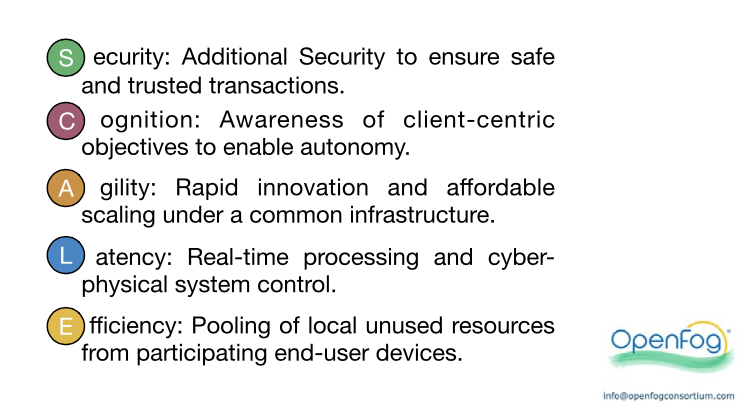
\includegraphics[width=.6\linewidth]{image/SCALE.png}
    \caption{SCALE}
    \caption*{img src: \cite{mukherjee2018survey}}
    \label{fig:scale}
\end{figure}

Fig. \ref{fig:pillars of openfog} shows the eight pillars of OpenFog. Fog nodes have several capabilities like storage, computation, networking, hardware, and software segments \cite{youtube}. \par

Security plays an important role in making systems trustworthy. And it is achieved with attestation, privacy, cryptographic techniques, and so on.
Scalability is incredibly important, especially within the IoT, where there might be billions of things to connect to IoT networks and also the fog.
And scalability makes sure that the system can control, configure, manage, orchestrate all of the capabilities and provides scalable performance. Openness is additionally important \cite{youtube}. 

\begin{figure}[H]
    \centering
    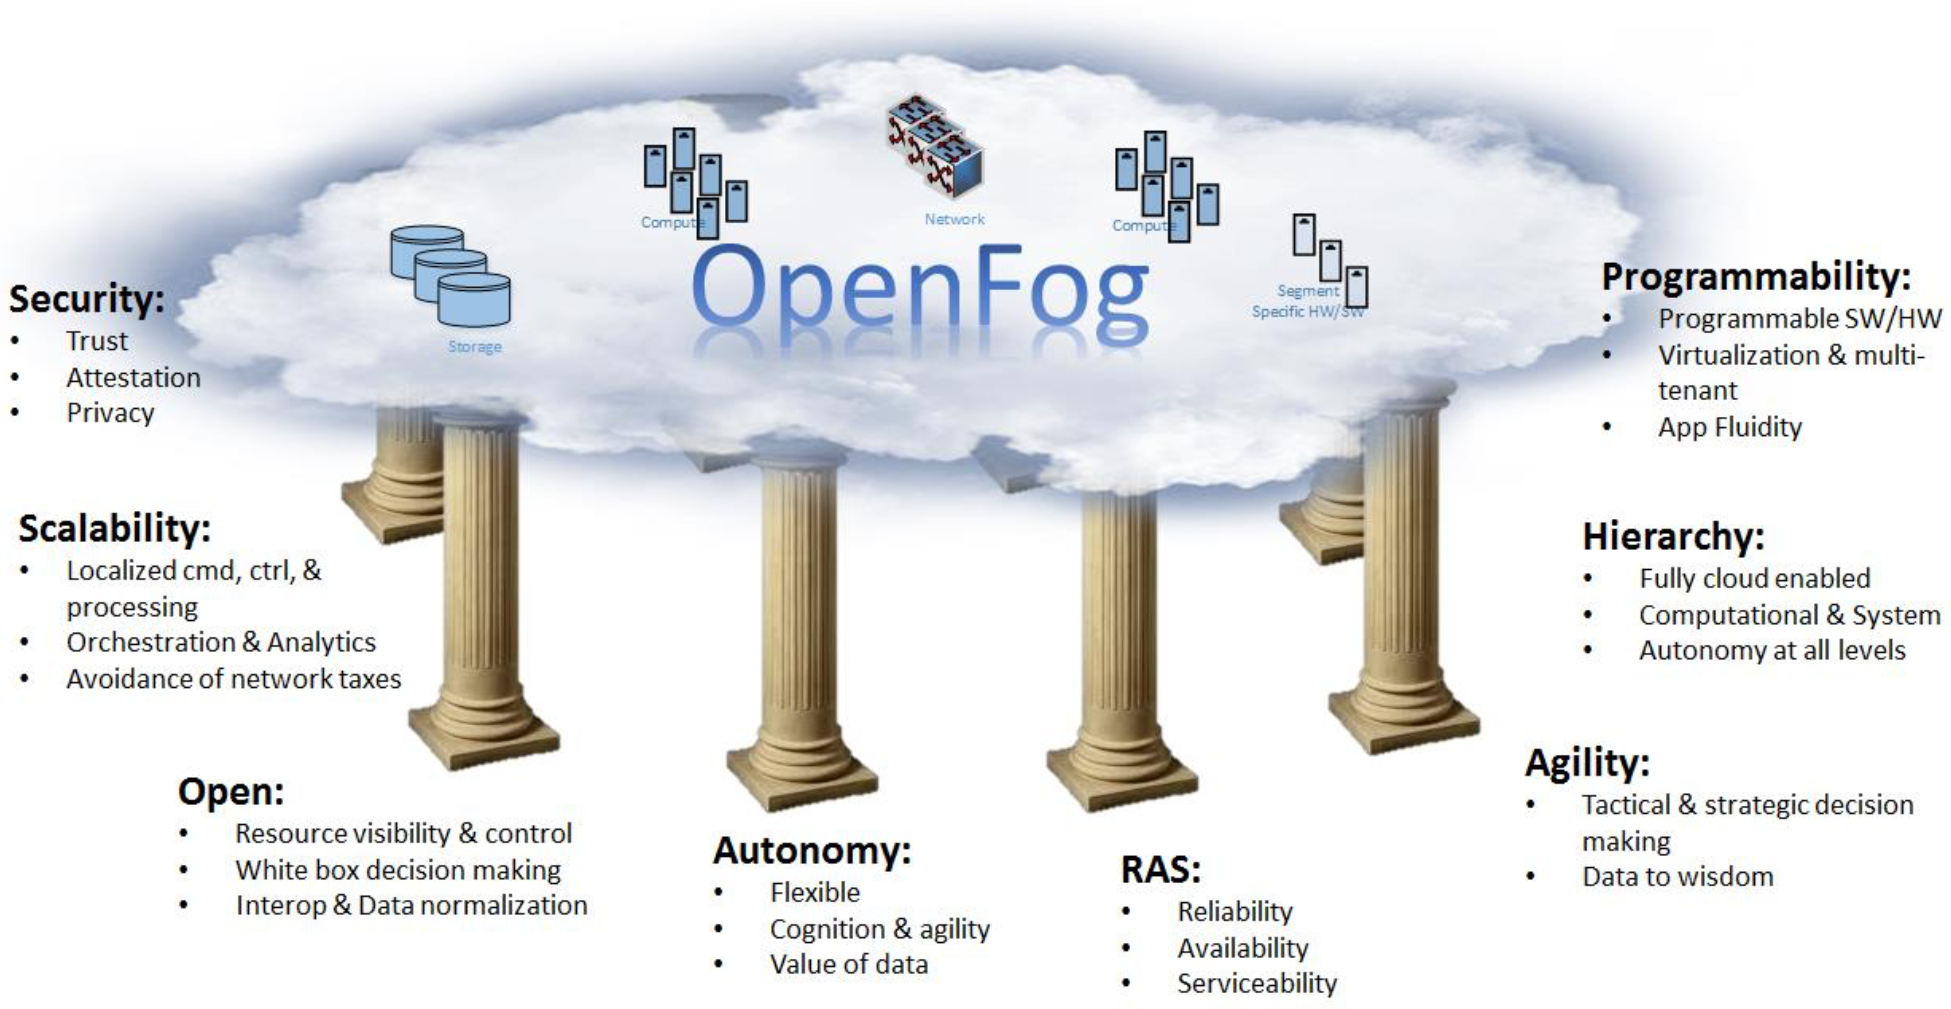
\includegraphics[width=\textwidth]{image/Pillars of OpenFog.png}
    \caption{Pillars of OpenFog}
    \caption*{img src: \cite{openfog2016openfog}}
    \label{fig:pillars of openfog}
\end{figure}

Fog nodes have to be autonomous, which means a fog network needs to be flexible and should be able to manage its cognitive abilities. 
RAS is a term for reliability, availability, and serviceability. It explains what fog does to keep itself reliable and trustworthy. 
Agility explains that a fog network should be able to make decisions tactically and strategically, which helps in converting data to wisdom or knowledge. 
Hierarchy explains that fog is fully cloud-enabled and distributes computational and system capabilities and also autonomous at all levels. 
Fog is a fully programmable architecture that provides programmable software and hardware capabilities, supports virtualization, multi-tenant operation, and app fluidity \cite{youtube}.

%------------------------------subsubsection2.3

\subsubsection{Main features of fog computing}

Fig. \ref{fig:scale} shows some of the advantages of fog computing like security, cognition, agility, latency, and efficiency \cite{openfog2016openfog}.

The main features of fog computing are \cite{mukherjee2018survey}, \cite{nat}, \cite{far}:
\begin{itemize}
    \item capacity of processing a high number of nodes,
    \item connection loss is impossible,
    \item end-device mobility,
    \item heterogeneity,
    \item low latency and location awareness,
    \item no bandwidth issues,
    \item privacy control,
    \item real-time applications,
    \item reduced operation costs,
    \item supports geographic distribution, and
    \item wireless access               
\end{itemize}

Fog computing is capable of processing a high number of nodes \cite{mukherjee2018survey}. Connection loss is impossible because of multiple interconnected channels \cite{nat}. Fog computing provides end-device mobility. Fog network connects heterogeneous devices irrespective of hardware and operating system \cite{madakam2018fog}. Fog computing can guarantee low latency and location awareness, as fog nodes are physically closer to the EU \cite{nat}, \cite{10.1145/3022636.3022649}. No bandwidth issues as data is fragmented and then combined while delivering \cite{nat}. Privacy control can be achieved by analyzing data locally instead of sending it to the cloud \cite{far}. Has endless capabilities to process real-time applications \cite{mukherjee2018survey}. Processing of preferred data locally, instead of sending it to the cloud, can save network bandwidth and also reduces operating costs \cite{far}. Fog computing supports geographic distribution and wireless access \cite{mukherjee2018survey}. 

%------------------------------subsubsection2.4

\subsubsection{Differences between cloud computing and fog computing}

The differences between cloud computing and fog computing \cite{mukherjee2018survey}, \cite{nat}, \cite{edu} are listed in Table \ref{tab:tab1} below.

\begin{center}
\begin{longtable}{|l|l|l|}
\caption{Comparison of cloud computing and fog computing} \label{tab:tab1} \\

\hline \multicolumn{1}{|c|}{\textbf{Features}} & \multicolumn{1}{c|}{\textbf{Cloud Computing}} & \multicolumn{1}{c|}{\textbf{Fog Computing}} \\ \hline 
\endfirsthead

\multicolumn{3}{c}%
{{\bfseries \tablename\ \thetable{} -- continued from previous page}} \\
\hline \multicolumn{1}{|c|}{\textbf{Features}} & \multicolumn{1}{c|}{\textbf{Cloud Computing}} & \multicolumn{1}{c|}{\textbf{Fog Computing}} \\ \hline  
\endhead

\hline \multicolumn{3}{|r|}{{Continued on next page}} \\ \hline
\endfoot

\hline \hline
\endlastfoot

%Access speed & Depends on VM & High\\
%Applications & Cyber-domain applications & Both Cyber-domain and cyber-physical applications, mainly time-critical applications\\
%Architecture & Centralized & Distributed\\
%Computing manner & Centralized & Both distributed and centralized\\
%Cost of deployment & High & Low\\
%Latency & High & Very low\\
%Maintenance & By technical experts & No human interference\\
%Mobility management & Easy & Hard\\
%Operation & By large companies & By both large and small companies depending on the size\\
%Reliability & High & Low\\
%Resource optimization & Global & Local\\
%Security & Low & Very high\\
%Size of DCs & Very large & Smaller\\

Access speed & Depends on VM & High\\
Architecture & Centralized & Distributed\\
Computing manner & Centralized & Both distributed and centralized\\
Cost of deployment & High & Low\\
Latency & High & Very low\\
Maintenance & By technical experts & No human interference\\
Mobility management & Easy & Hard\\
Reliability & High & Low\\
Resource optimization & Global & Local\\
Security & Low & Very high\\
Size & Very large & Smaller\\

\end{longtable}
\end{center}

Cloud computing supports cyber-domain applications. Whereas, fog computing supports both cyber-domain and cyber-physical applications, mainly time-critical applications.  Cloud is operated by large companies and fog is operated by both large and small companies depending on the size. Even though fog computing provides low latency, cloud computing is more reliable than fog computing. The size of cloud DCs is very large and the size of the fog system is smaller. But, multiple smaller fog nodes form a large fog system \cite{mukherjee2018survey}.

%------------------------------subsubsection2.5

\subsubsection{Fog architecture}

Fog architecture consists of a number of different layers. The most commonly used architectures in fog computing are three-tier architecture and layered architecture. The architectures are discussed in Sec. \ref{sec:3}

%-----------------------------------------------------------------subsection3

\subsection{Cloud Computing}

%------------------------------subsubsection3.1

\subsubsection{Definition}

According to \cite{mell2011nist} "Cloud computing is a model for enabling ubiquitous, convenient, on-demand network access to a shared pool of configurable computing resources (e.g., networks, servers, storage, applications, and services) that can be rapidly provisioned and released with minimal management effort or service provider interaction. This cloud model is composed of five essential characteristics, three service models, and four deployment models.

\begin{itemize}
    \item Essential characteristics: On-demand self-service, broad network access, resource pooling, rapid elasticity, measured service.
    \item Service models: Software as a Service (SaaS), Platform as a Service (PaaS), Infrastructure as a Service (IaaS).
    \item Deployment models: Private cloud, community cloud, public cloud, hybrid cloud."
\end{itemize}

%------------------------------subsubsection3.2

\subsubsection{Service-oriented distributed computing in the cloud}

The objectives are computing, storage, networking, and management on demand (U. Krieger: KTR-Mobicom-M-E). \par
Scalable distributed computing using characteristics like resource pooling. Unlimited storage capacity. The connection between applications and servers is by IP networks (U. Krieger: KTR-Mobicom-M-E). 

%------------------------------subsubsection3.3

\subsubsection{Virtualization}

Types of virtualization in cloud computing are application, network, desktop, and storage virtualization \cite{nam}. \par
The basic virtualization technologies are Virtual Machine (VM) and Docker. \par
A VM also known as a hypervisor is a software or hardware that creates and runs virtual machines \cite{hypervisor}.
A VM imitates the actions of the computer. It runs in the dedicated window and leaves the user with the experience of using the host system. It runs in its own sandbox. Many VMs can run at the same time on the host system. Each VM has it's own OS and shares the hardware of the host system for VM support. The abstraction of hardware reduces costs and  power demand \cite{mic}. 

"Docker allows you to package an application with all of its dependencies into a standardized unit for software development" (Dr. Andreas Schönberger, Großmann, Dr. Kolb, Manner DSG-SOA-M 2020 – 9 – Docker). "Docker containers wrap up a piece of software in a complete filesystem that contains everything it needs to run: code, runtime, system tools, system libraries - anything you can install on a server. This guarantees that it will always run the same, regardless of the environment it is running in" (Dr. Andreas Schönberger, Großmann, Dr. Kolb, Manner DSG-SOA-M 2020 – 9 – Docker). Docker works on build, ship, and run everywhere paradigm (Dr. Andreas Schönberger, Großmann, Dr. Kolb, Manner DSG-SOA-M 2020 – 9 – Docker). The process of deploying applications with the help of containers is called containerization. Containers are flexible, lightweight, loosely coupled, portable, scalable, and secure \cite{doc}. \par

\begin{figure}[H]
    \centering
    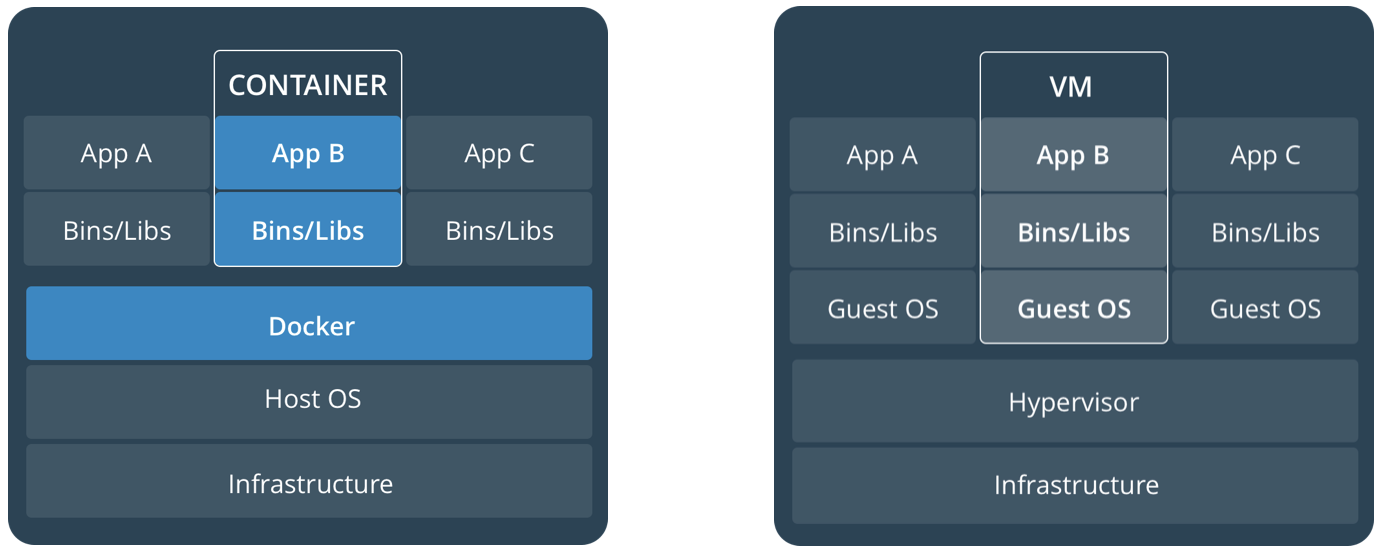
\includegraphics[width=\textwidth]{image/Containers and virtual machines.png}
    \caption{Containers and virtual machines}
    \caption*{img src: \cite{doc}}
    \label{fig:containers and virtual machines}
\end{figure}

Docker containers are lightweight and easy to manage as they share the host OS for isolation support. Besides, VMs are heavy as each VM has its own guest OS. Docker containers are preferred when users have to deploy multiple applications over a single host OS. On the other hand, VMs are preferred when the users have to run applications on different OSs \cite{doc}, \cite{avi}. 

%-----------------------------------------------------------------subsection4

\subsection{Virtualized Fog DCs}

According to \cite{wiki:xxx} "Data center is a pool of resources (computational, storage, network) interconnected using a communication network. Data Center Network (DCN) holds a pivot role in a data center, as it interconnects all of the data center resources together." A DCN is defined by its network topology, protocols, and routing/switching equipment \cite{mukherjee2018survey}. Types of DCN are Three-tier DCN, Fat tree DCN, and Dcell \cite{wiki:xxx}. \par
Fig. \ref{fig:data center virtualization} shows data center virtualization where multiple Virtual Networks (VNs) can be created and implemented independently. VNs can be processed in isolation as they are independent of each other. All the resources are virtualized  in a virtual data center with the help of a hypervisor which makes application deployment easier \cite{mukherjee2018survey}. \par

Server virtualized technologies like VMware and Xen can support the requirements of traditional data centers like high server utilization, performance isolation, and low operation costs. But, they cannot support application deployment, flexibility, and security related issues. So, the main goal of data center virtualization is to address flexibility and efficiency to meet the requirements of Data Service Subscribers (DSSs). Based on the requirements of DSSs, Massive Data Center Operators create (MDCO) a virtualized server \cite{mukherjee2018survey}. 

\begin{figure}[H]
    \centering
    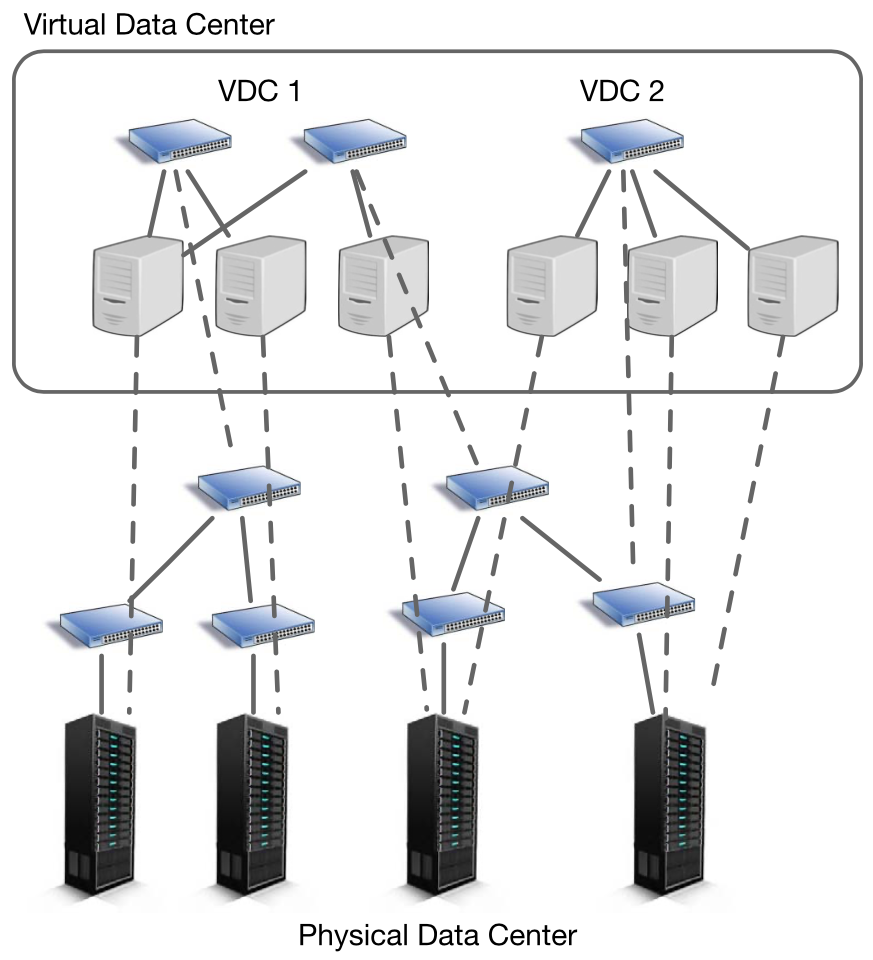
\includegraphics[width=.5\linewidth]{image/Data center virtualization.png}
    \caption{Data center virtualization}
    \caption*{img src: \cite{mukherjee2018survey}}
    \label{fig:data center virtualization}
\end{figure}

One server alone can process the requirements of DSSs, which improves capacity utilization and energy efficiency. Even though a single server can process requirements of multiple DSSs, as massive data centers and DSSs are far from each other, massive data centers may encounter high latency and operation costs. As a solution, fog computing supports multiple virtualized edge data centers to offload the service from massive data centers \cite{mukherjee2018survey}. \par

Fig. \ref{fig:data center networks with fog computing} shows the three-tier architecture where the bottom tier consists of DSSs, the middle tier consists of MDCOs, and the top tier consists of FNs. FNs and MDCOs share computation and storage facilities. And, MDCOs provide latency-sensitive services to the DSSs \cite{mukherjee2018survey}.

\begin{figure}[H]
    \centering
    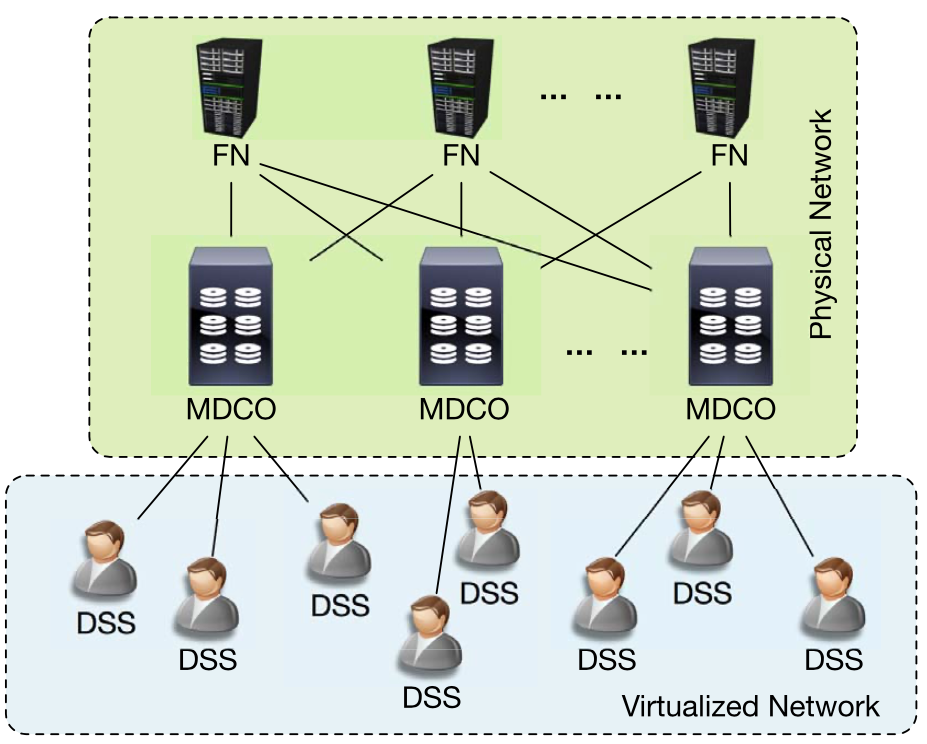
\includegraphics[width=.5\linewidth]{image/Data center networks with fog computing.png}
    \caption{Data center networks with fog computing}
    \caption*{img src: \cite{mukherjee2018survey}}
    \label{fig:data center networks with fog computing}
\end{figure}
\section{Fog Computing-Based Architectures}
\label{sec:3}

%-----------------------------------------------------------------subsection1

\subsection{Architecture}

The architecture explains how fog computing extends services offered by the cloud i.e., computation, communication, and storage to the edge of the network \cite{mukherjee2018survey}.

%------------------------------subsubsection1.1

\subsubsection{Three-tier architecture}

Fig. \ref{fig:three-tier fog computing architecture} shows the three-tier architecture which is broadly used among all the architectures of fog computing \cite{mukherjee2018survey}. \par

The bottom tier consists of end devices such as IoT devices, sensor nodes, smart devices, and so on. These end devices are also known as Terminal Nodes (TNs) \cite{mukherjee2018survey}. These nodes can sense and capture the data \cite{webpage} and are equipped with Global Positioning System (GPS) \cite{mukherjee2018survey}. TNs are heterogeneous that work irrespective of technology, communication mode, hardware, and OS \cite{webpage}. \par

\begin{figure}[H]
    \centering
    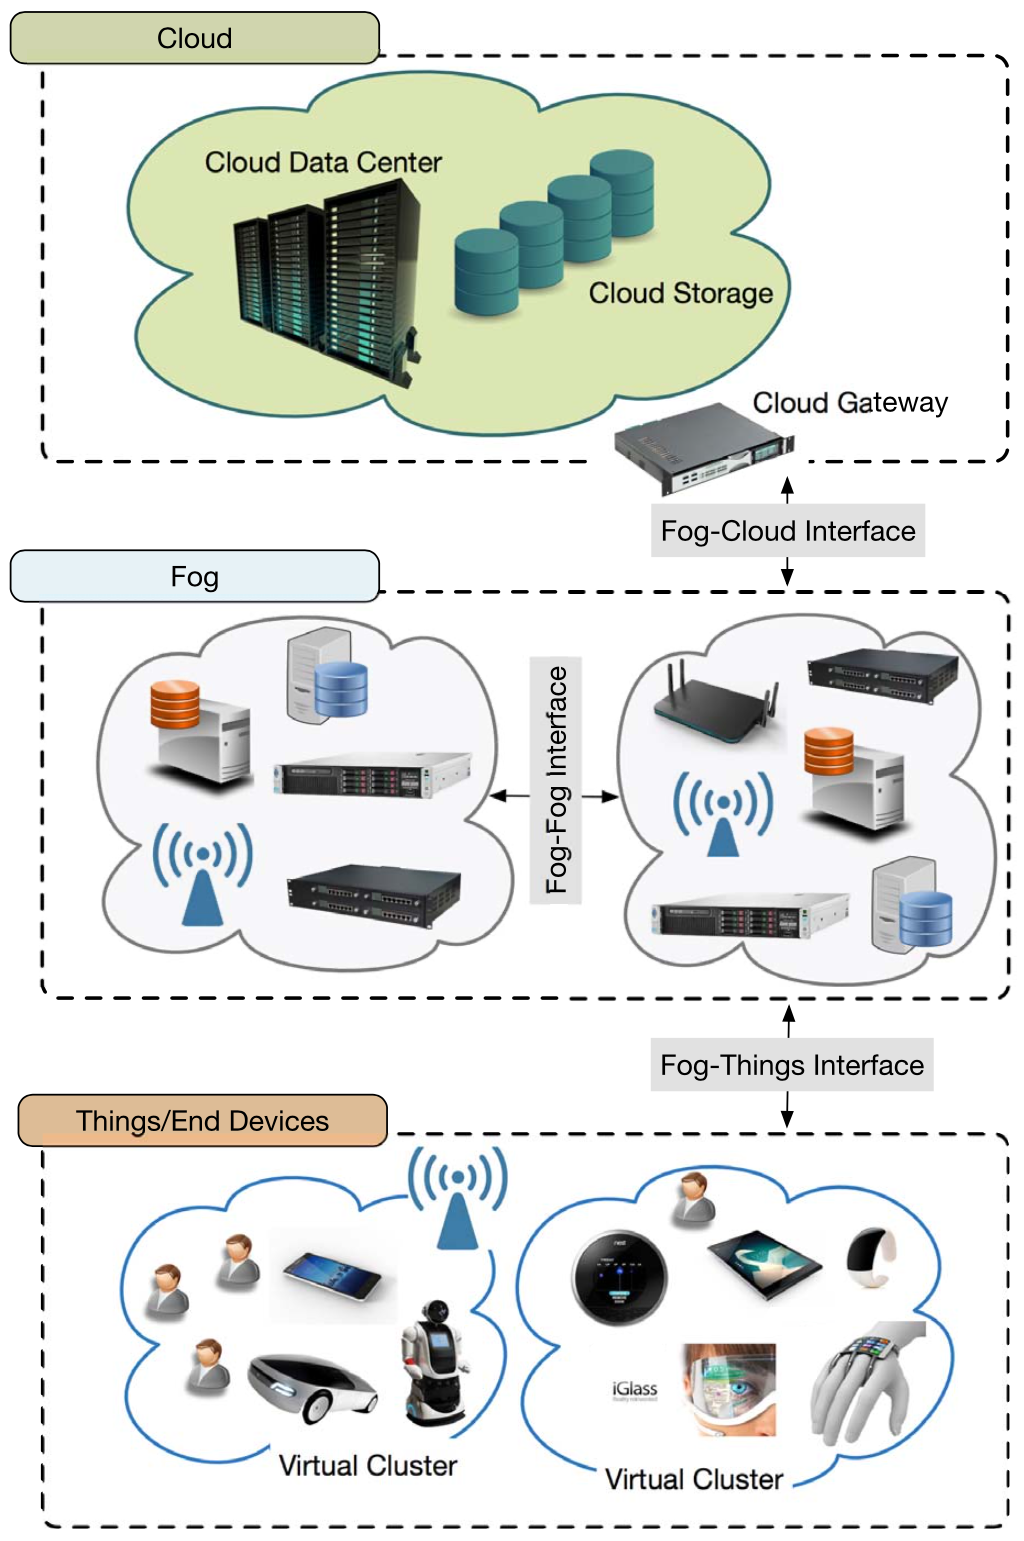
\includegraphics[width=.5\linewidth]{image/Three-tier fog computing architecture.png}
    \caption{Three-tier fog computing architecture}
    \caption*{img src: \cite{mukherjee2018survey}}
    \label{fig:three-tier fog computing architecture}
\end{figure}

The fog tier is known as the fog computing layer which consists of network devices like routers, gateways, switches, Access Points (APs), base stations, fog servers, and so on \cite{mukherjee2018survey}, \cite{webpage}. These devices are also called fog nodes \cite{mukherjee2018survey}. Fog nodes are static \cite{webpage} and provide computation and storage facilities to the end devices \cite{mukherjee2018survey} and are positioned in between end devices and DCs \cite{webpage}. \par

The top tier is the cloud which consists of traditional cloud servers, cloud DCs, sufficient storage, and computing facilities \cite{mukherjee2018survey}. This tier has powerful computation and high storage capabilities also provide permanent storage and act as back-up \cite{webpage}. 

%------------------------------subsubsection1.2

\subsubsection{Layered architecture}

Fig. \ref{fig:layered architecture for fog computing} shows the layered architecture for fog computing which contains physical and virtualization, monitoring, preprocessing, temporary storage, security, and transport layers \cite{mukherjee2018survey}.

The physical and virtualization layer consists of physical and virtual nodes which are responsible for data collection \cite{mukherjee2018survey}, \cite{webpage}. And the collected data is sent to the further layers for processing \cite{webpage}.\par

The monitoring layer monitors the nodes, handles service requests, and checks the node's energy consumption issues \cite{mukherjee2018survey}, \cite{webpage}. \par

The preprocessing layer manages data by performing data analysis operations \cite{webpage} such as data filtering and trimming \cite{mukherjee2018survey}. Data should be analyzed before using so that unwanted data can be removed and necessary data can be preserved \cite{webpage}. \par

\begin{figure}[H]
    \centering
    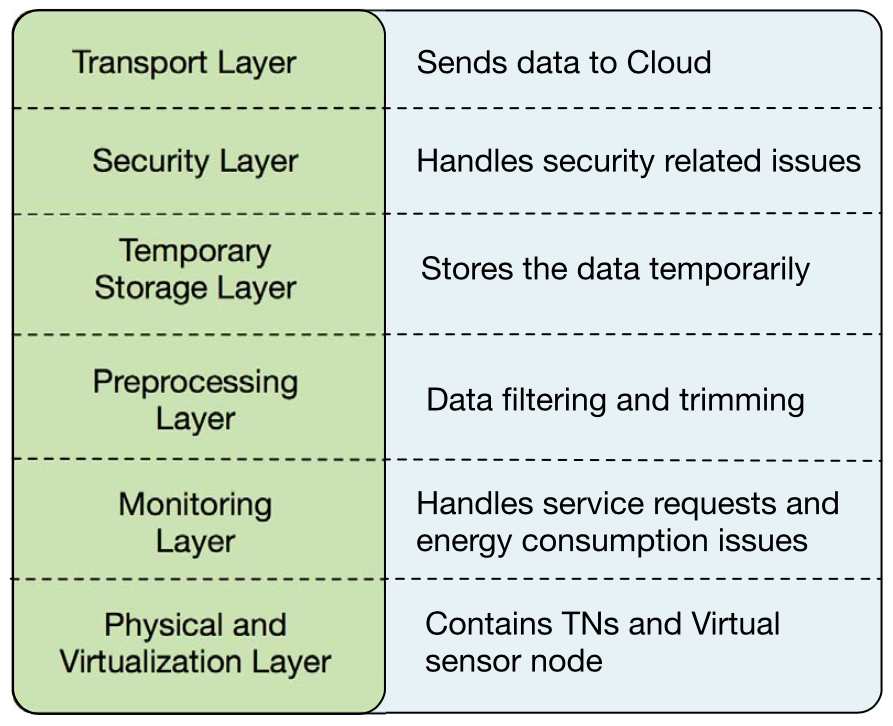
\includegraphics[width=.5\linewidth]{image/Layered architecture for fog computing.png}
    \caption{Layered architecture for fog computing}
    \caption*{img src: \cite{mukherjee2018survey}}
    \label{fig:layered architecture for fog computing}
\end{figure}

The temporary storage layer stores the data temporarily \cite{mukherjee2018survey} as a replica with the help of virtual storage before moving it to the cloud \cite{webpage}. Once the data is sent to the cloud, temporary data stored in this layer will be removed \cite{webpage}. \par

The security layer handles all the issues related to security \cite{mukherjee2018survey}. Ensures privacy, integrity, encryption, and decryption of the data \cite{webpage}. \par

The transport layer sends the data to the cloud \cite{mukherjee2018survey} for permanent storage \cite{webpage}. To achieve efficiency only part of the data is sent to the cloud \cite{webpage}.

%-----------------------------------------------------------------subsection2

\subsection{Networking}

%------------------------------subsubsection2.1

\subsubsection{Fog computing architecture using Software-Defined Networking (SDN)}

Integrated hardware and software are used for conventional networking to direct traffic through a series of routers and switches \cite{yt}. According to \cite{mukherjee2018survey} "Software-Defined Networking (SDN), is an emerging solution that provides a flexible way to update and reconfigure the network." The main idea behind SDN is to virtualize the network \cite{yt} by separating the control plane and the data plane \cite{mukherjee2018survey}. The control plane manages the network and the data plane is where the traffic flows \cite{yt}. OpenFlow is an open protocol between the control plane and data plane \cite{mukherjee2018survey}, that enables the server to tell network switches where to send packets \cite{marg}. The centralized controller called the SDN controller \cite{mukherjee2018survey} manages all the network traffic \cite{yt} and also handles packet forwarding and other networking functionalities \cite{mukherjee2018survey}. The SDN controllers communicate with switches by establishing a TCP connection. The delay between the SDN controller and the switch is a drawback. And the distributed controller might be a solution for this. But, it does increase the number of controllers as there will be one controller per network, which results in a one-hop delay. One solution is the authority switch, which shares the functions of the controller \cite{mukherjee2018survey}. \par

\begin{figure}[H]
    \centering
    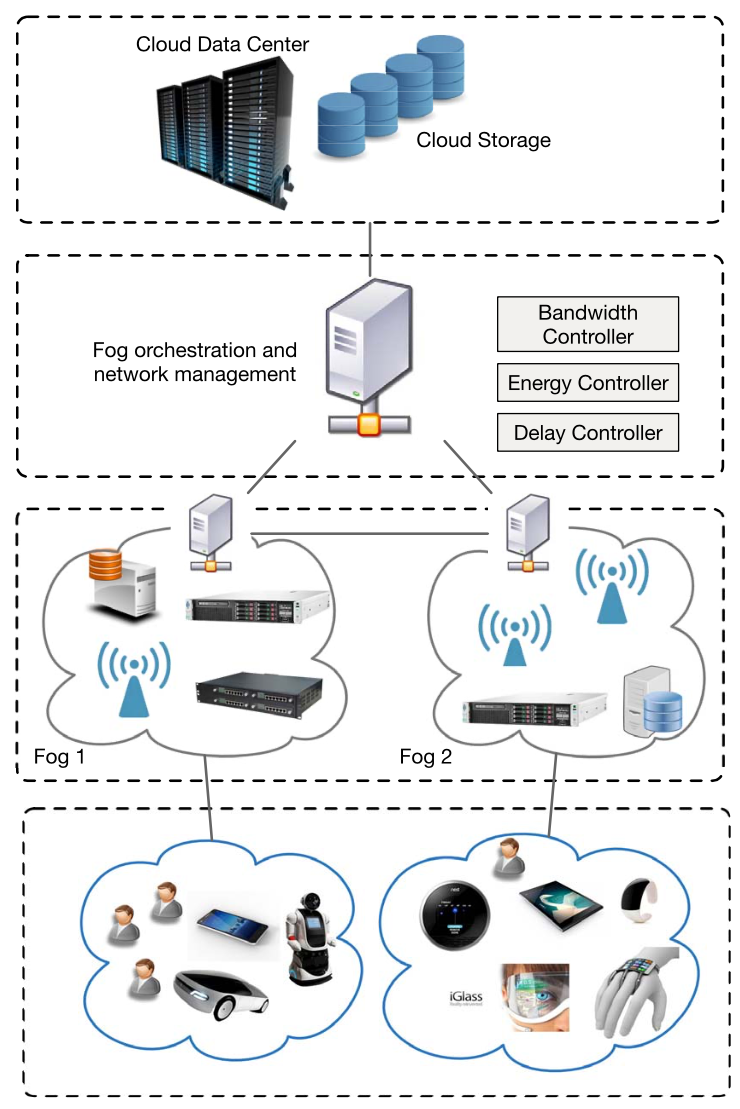
\includegraphics[width=.5\linewidth]{image/SDN-based fog computing architecture.png}
    \caption{SDN-based fog computing architecture}
    \caption*{img src: \cite{mukherjee2018survey}}
    \label{fig:sdn-based fog computing architecture}
\end{figure}

Fog computing is the best approach to provide latency-sensitive services. Even though it is the best option, due to the mobility issues of end devices and traffic distribution, there may be a shortage of available fog computing resources. So, if there are not enough resources in the fog layer, it would be better to transfer some of the latency-aware fog tasks to the cloud. Then, SDN will be aware of the network state and distributes the latency-aware fog tasks. Additionally, dynamic QoS policy deployment is required to handle fog services with different QoS. So, it is important to offer software-defined QoS in fog computing. Therefore, computation and the transmission load on the SDN controller can be minimized. And in SDN-implemented fog networks, scalability and resource management can be improved \cite{mukherjee2018survey}.

Fig. \ref{fig:sdn-based fog computing architecture} shows the SDN-based fog computing architecture. The fog-SDN controller that supports dynamic QoS distinguishes the SDN based architecture from the conventional three-tier architecture of the fog computing. The SDN controller layer defines the QoS based on the attributes and state of the data of the fog node. To get an SDN-based fog computing system, the SDN controller has to support virtualization. To support virtualization, the SDN controller has to be implemented with a hypervisor \cite{mukherjee2018survey}. \par

Fig. \ref{fig:the components of fog-SDN controller} shows the necessary hardware and software components of the fog-SDN controller \cite{mukherjee2018survey}. \par

\begin{figure}[H]
    \centering
    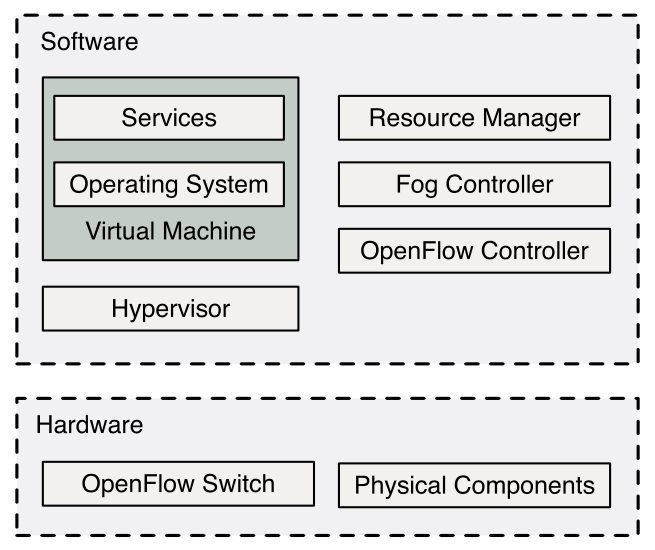
\includegraphics[width=.5\linewidth]{image/The components of fog-SDN controller.png}
    \caption{The components of fog-SDN controller}
    \caption*{img src: \cite{mukherjee2018survey}}
    \label{fig:the components of fog-SDN controller}
\end{figure}

The key concept of SDN is that SDN controllers act as fog orchestration and resource manager \cite{mukherjee2018survey}. \par

According to \cite{sdx} 'SDN orchestration' is "The ability to program automated behaviors in a network to coordinate the required networking hardware and software elements to support applications and services." \par

The fog computing architecture is implemented at edge switches using SDN. It is hard to implement fog computing at switches due to the centralized nature of SDN. So, the controller functionality is integrated at edge switches to perform discrete and distributed computation. Message Queuing Telemetry Transport (MQTT) is used as an IoT protocol for implementation \cite{mukherjee2018survey}.  

Fig. \ref{fig:sdn-based fog (switch) node} shows the framework proposed in \cite{xu2016sdn} to identify and dock/undock applications without EUs interference. The main goal of this framework is to efficiently handle the storage, computation, and networking resources of switches and provide flexibility to SDN by bringing them to the edge of the network. 
The two main components in Fig. \ref{fig:sdn-based fog (switch) node} are Open vSwitch (OvS) and docker management application. The OvS provides a virtual network bridge between individual applications. And it has an SDN controller that handles packet forwarding and other networking functionalities. A virtual Ethernet connection establishes a connection between OvS and docker management application. This framework initiates the flow and manages UEs requests and a pool of applications.

\begin{figure}[H]
    \centering
    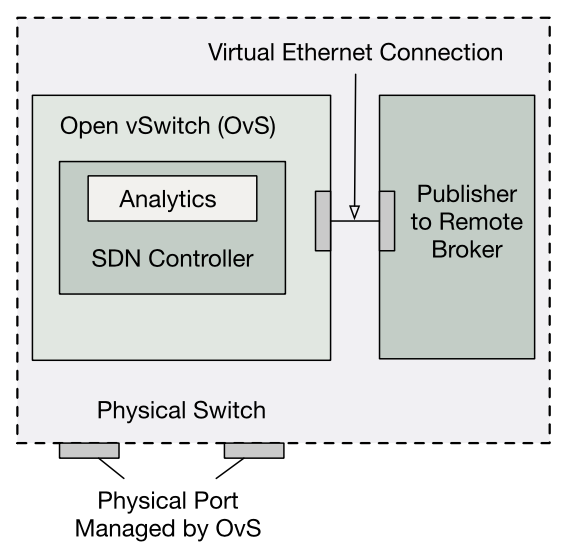
\includegraphics[width=.5\linewidth]{image/SDN-based fog (switch) node.png}
    \caption{SDN-based fog (switch) node}
    \caption*{img src: \cite{mukherjee2018survey}}
    \label{fig:sdn-based fog (switch) node}
\end{figure}

%------------------------------subsubsection2.2

\subsubsection{Fog-Radio Access Networks (F-RANs)}

Radio Access Network (RAN) is a part of cellular technology that establishes a connection between User Equipment (UE) and Core Network (CN) \cite{wi}. It was not easy to manage distributed sites using RAN. So, Cloud-Radio Access Network (C-RAN) was introduced \cite{rf}.  \par 

C-RAN is a centralized architecture for RANs based on cloud computing \cite{mar}. It supports 2G, 3G, 4G \cite{w}, and future wireless communication technologies like 5G and IoT \cite{mar}. C-RAN is also known as Centralized-RAN \cite{w}. The components of C-RAN are Remote Radio Head (RRH), Baseband Unit (BBU) pool, and Mobile Switching Center (MSC). RRH transmits signals, the BBU pool is a central station that processes data, and MSC establishes a connection to the users. Fronthaul connects the BBU pool and RRHs \cite{guizani2017cran}. Backhaul connects the BBU pool to the CN using optical fiber \cite{raj}. \par

Due to the centralized architecture of C-RAN, it is difficult to manage the mobility of users and increased data demand. That increases the burden on fronthaul. To address these issues, Heterogeneous-Cloud Radio Access Network (H-CRAN) which is more efficient than C-RAN was introduced \cite{zhang2017fog}. Instead of the BBU pool, High Power Nodes (HPNs) acts as a central station and does processing in H-CRAN. Fronthaul just transfers the data, and backhaul connects HPNs to the BBU Pools \cite{guizani2017cran}. \par

Fog-Radio Access network (F-RAN) is a hybrid architecture that combines the benefits of H-CRAN and FogNet \cite{mukherjee2018survey}. F-RAN extends resource management, signal processing, distributed storage, and caching capabilities to the edge of the network \cite{zhang2017fog}. The components of F-RAN are Fog-Access Points (F-APs) and Fog-User Equipment (F-UE). F-APs and F-UE do signal processing, have caching capabilities, and Radio Resource Management (RRM) functionalities \cite{guizani2017cran}. Data can be retrieved in this hybrid model in three ways: directly from users, cached at the BBU pool, and from cloud network \cite{mukherjee2018survey}. \par

\begin{figure}[H]
    \centering
    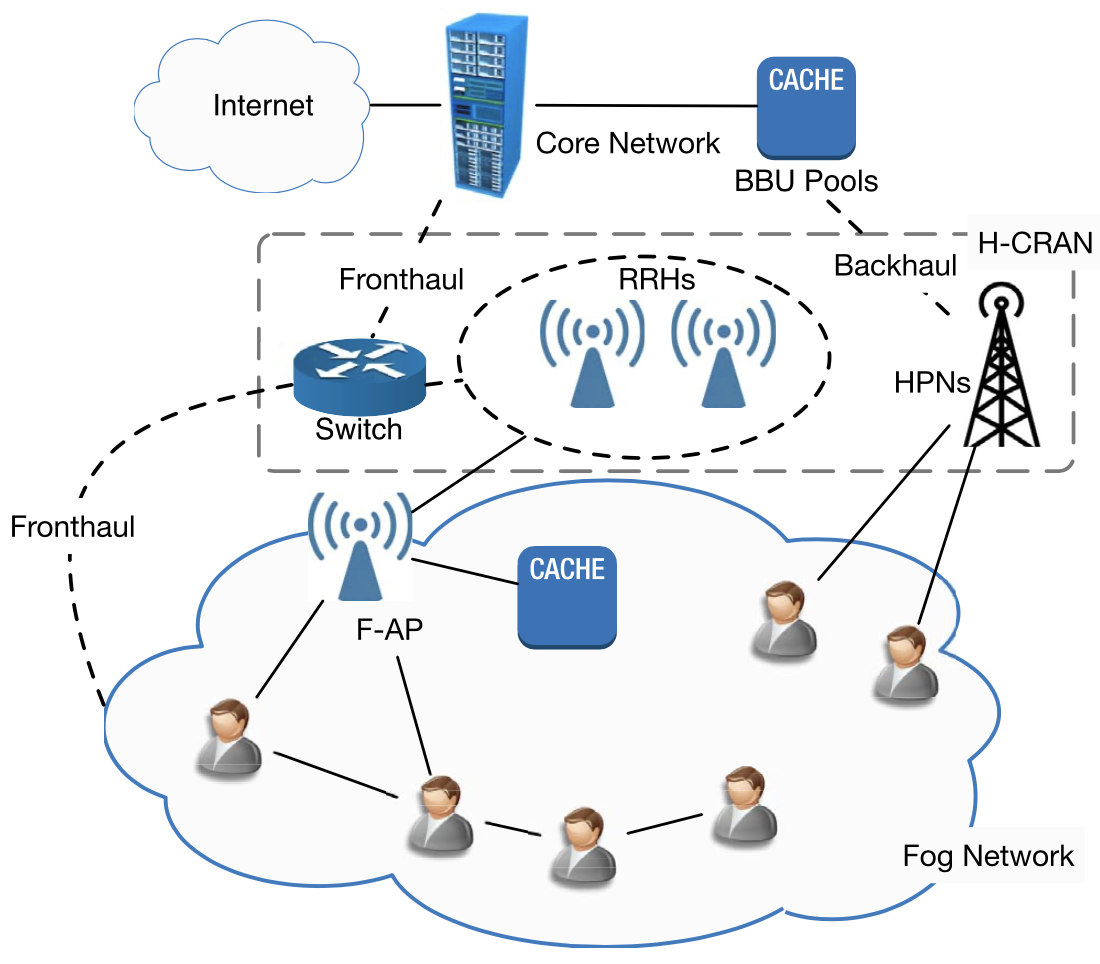
\includegraphics[width=.5\linewidth]{image/FogNet or H-CRAN architecture.png}
    \caption{FogNet/H-CRAN architecture}
    \caption*{img src: \cite{mukherjee2018survey}}
    \label{fig:fognet/h-cran architecture}
\end{figure}

Challenges of F-RAN are \cite{guizani2017cran}:
\begin{itemize}
    \item To support large-scale users and services, the F-RAN requires further research to expand the storage capabilities of both F-APs and F-UEs. Thus, coordinated caching policies for different F-APs and F-UEs need to be ensured \cite{guizani2017cran}.
    \item Implementing SDN is another challenge as an edge network is distributed architecture. Also, the SDN controller is placed in the BBU pool, and fronthaul transfers the data which makes it worse \cite{guizani2017cran}.
\end{itemize}

User access modes:
 \begin{itemize}
    \item D2D mode: D2D mode is selected, when the user requesting the data supports D2D mode, and the requested data is provided by another D2D-enabled user within a predefined distance and the Signal-to-Interference Ratio (SIR) of both the users is greater than the SIR threshold \cite{mukherjee2018survey}.
    \item Nearest F-AP mode: User requesting the data needs access to F-APs if the user does not support D2D mode, and requested data is not available at another D2D-enabled user, and SIR is not greater than threshold \cite{mukherjee2018survey}. 
    \item Local distributed co-ordinated mode: Here, the user requesting the data is connected to multiple F-APs in a user-centric cluster. F-RAN regulates the radius of the cluster to satisfy SIR \cite{mukherjee2018survey}. 
\end{itemize}

%------------------------------subsubsection2.3

\subsubsection{Caching and Offloading}

One of the vital challenges in F-RAN is file caching. Uncoded and coded caching are two caching strategies. The complete file is cached in uncoded caching. But, in coded caching fragments of files are cached in multiple caches using Maximum Distance Separable (MDS) code. RRH caches files until it ran out of memory and processes requests of EUs without using backhaul. But, there will be a burden on backhaul because of the uncached files. So, there should be more number of RRHs for uncached file sharing and less power consumption, and less number of Radio Units (RUs) to reduce the burden on the backhaul. But, due to a lack of cooperation, there will be an increase in power consumption \cite{mukherjee2018survey}. 

\begin{figure}[H]
    \centering
    \includegraphics[width=.5\linewidth]{image/caching policy.png}
    \caption{Caching policy}
    \caption*{img src: \cite{mukherjee2018survey}}
    \label{fig:caching policy}
\end{figure}

In F-RAN, prefetching and delivery are two phases for arbitrary caching. If content popularity is the same, then in prefetching phase processing is done with multiple transmission intervals. But, in the delivery phase on one of the transmission intervals. This depends on data cached during the prefetching phase. Hard and soft-transfer mode are two fronthaul-aware approaches. In hard-transfer mode, data that was not found in the local server was sent from BBU to RRHs. In soft-transfer mode, the quantized version of the baseband signal encoded at BBU is sent to RRHs \cite{mukherjee2018survey}. 
\section{Applications and Usage of Fog Computing}

\begin{figure}[H]
    \centering
    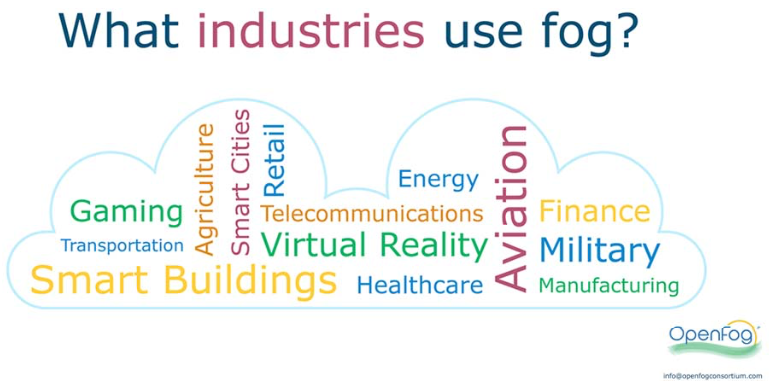
\includegraphics[width=.5\linewidth]{image/Applications of fog computing.png}
    \caption{Applications of fog computing}
    \caption*{img src: \cite{mukherjee2018survey}}
    \label{fig:applications of fog computing}
\end{figure}

Fog computing is the best approach to support geographically distributed, latency-sensitive, and QoS-aware IoT applications. It has a huge potential to meet the requirements of various applications like smart cities, healthcare, agriculture, aviation, energy, finance, gaming, manufacturing, military, retail, smart building, telecommunications, transportation, and virtual reality \cite{mukherjee2018survey}. Some are discussed below.

%-----------------------------------------------------------------subsection1

\subsection{Smart cities}

The major challenge of smart cities is the increased data demand and the number of IoT devices connected to the network. It is really hard to manage and keep track of the data generated. And also transferring this vast data between cloud and DCs causes delay, and effects communication costs \cite{sandra}. \par

Using fog computing, the amount of data sent to the cloud for processing can be reduced. This improves efficiency. There are many advantages by using fog computing for smart cities \cite{sandra}. \par

\begin{itemize}
    \item A minimal amount of data is sent to the cloud:  Instead of sending all the data to the cloud, fog manages the amount of data to be sent to the cloud. All the devices connected to the network generate a huge amount of data \cite{sandra}. And fog manages this data by performing data analysis operations \cite{webpage} like data filtering and trimming in the preprocessing layer \cite{mukherjee2018survey}, \cite{sandra}. Data is analyzed before sending it to the cloud so that unwanted data can be removed  and necessary data can be preserved \cite{webpage}, \cite{sandra}.
    \item Low latency: Fog nodes are capable of processing the data instead of sending it to the cloud. This saves the time of data being sent to the cloud and waiting for the response \cite{sandra}. As fog nodes are geographically much closer to the EUs than DCs, it is appropriate for latency-sensitive, and time-sensitive requests \cite{mukherjee2018survey}.
    \item Reduced bandwidth: Processing and transferring the data over the network demands high bandwidth. As data is distributed between the end devices in the fog it reduces the bandwidth consumption \cite{sandra}. 
    \item Better security: Data security is very important in any application, as sensitive and confidential data will be sent over the communication channels \cite{sandra}. Fog ensures better security with privacy, attestation, cryptographic techniques, and so on \cite{youtube}.
\end{itemize}

According to \cite{sandra}, smart cities is the best area to implement fog computing. As millions of things in the city are connected across the network they produce heterogeneous data of different aspects like air quality, public safety, road traffic, surveillance, waste management, and so on. Fog computing makes sure that all the data generated is managed and processed effectively \cite{sandra}. Some of the aspects are discussed below.

\begin{itemize}
    \item Traffic control: Different kinds of sensors are used to monitor and control traffic. Sensors can detect pedestrians, bikers, and drivers by measuring their speed of motion and the relative distance between them. The data collected in real-time is analyzed and decisions were made accordingly. For e.g. changing the colour of traffic lights \cite{sandra}. And video camera which can detect the flashlight of emergency services vehicles like ambulance, and fire trucks and changes the lights to clear the roads \cite{waheetha2016fog}.
    \item Waste management: This process requires a lot of time, money, and resources. Traditionally, each city will its have own schedule for garbage collection. Every household in the city keeps its bins outside for garbage collection on a specific day as mentioned in the schedule. Some bins will be empty and some overfilled. This results in a waste of resources and manpower as every household don't have an equal amount of waste. And some people might forget or will be unaware of garbage collection even though they have huge waste to be disposed of. And they should wait for the next possible day of garbage collection. The integration of sensors and fog computing supports real-time monitoring of garbage. By installing sensors in garbage bins they will notify users to change the bin if it's full. And by collecting all the garbage data of the whole city schedules can be optimized \cite{sandra}.
    \item Surveillance: Surveillance systems generate a huge amount of data. As fog nodes are closer to the EUs they capture and process the data quickly. The low latency feature of fog provides effective surveillance. This helps to detect violence in public places in real-time and situations where security, police, and fire services are necessary \cite{sandra}.
\end{itemize}

%-----------------------------------------------------------------subsection2

\subsection{Healthcare}

The main idea behind healthcare IoT is to make it easier for patients to consult their doctors anytime, anywhere possible. But the healthcare system encounters some challenges like processing of big data, the geographic distribution of users, privacy and security. So, fog computing is the best approach for healthcare IoT \cite{jennifer}. \par

As mentioned above fog is capable of processing big data by performing data analysis operations \cite{webpage} and fog nodes can process data instead of sending it to the cloud \cite{sandra}. Fog ensures privacy and security with predefined authorization techniques and exposes data through a secured channel. Only an authorized person can hold the data and make changes to it. Instead of sending health records every time, users can provide access to doctors, pharmacies, and other healthcare personnel so that they can have a real-time update of the user's condition \cite{jennifer}. \par

Sensor installed devices can be used as wearables to monitor patient's condition e.g. blood pressure, heart rate, and many more. These smart devices can also remind users about their physical activity. These are life savior for elderly people who live alone. Any change in the patient's condition alerts the doctor and people related to him/her. Data collected from these devices helps a doctor to monitor patients from time to time. And, sensor installed devices can also be used to track the location of the medical equipment in hospitals like wheelchairs, oxygen pumps, stretchers, and so on. Besides, sensor installed devices can also be used to monitor temperature, and humidity \cite{dr}. 

Healthcare IoT using fog computing reduces costs as one can monitor the patient's condition in real-time. No unnecessary visits to the hospitals which saves time and resources. Continuous monitoring helps doctors to diagnose patient's problems earlier \cite{dr}. 
\section{Conclusion}

Fog computing is not a replacement but an extension of cloud computing. Computation, communication, and storage functionalities of cloud computing are extended to the edge of the network. Fog computing supports geographically distributed, latency-sensitive, and QoS-aware IoT applications. It has a huge potential to process time-sensitive service requests. Fog computing is the best alternative, but it does have some limitations. Application offloading, lack of resources, mobility, F-RANs, heterogeneity, and SDN-Based fog computing address challenges of fog computing. Fog computing can be applied to a wide range of next-generation network applications.
%
%===============================================================================
% LATEX-Dokument: Literaturverzeichnis
%===============================================================================
%
\newpage
\phantomsection
% Einstellungen f\"{u}r Literaturverzeichnis
\addcontentsline{toc}{section}{\bibname}

\bibliographystyle{IEEEtran}
% argument is your BibTeX string definitions and bibliography database(s)
\bibliography{literature/bib}
% Nutzung von Bibtex:
% hier den bib-file einbinden
%
% GATHER{bibfile.bib}
% \footnotesize
% \bibliography{bibfile}
% ansonsten: bbl als tex Datei einbinden
 %\input{KTR-Seminar-Literatur.tex}
%===============================================================================
% LATEX-Dokument: Literaturverzeichnis
%===============================================================================
%
\end{document}
